\section{Tables and Chairs with Correlated Random Prices}

In this final stage of the tables and chairs example we introduce
correlated random prices. We follow economic practice by developing a
small story around the problem to tie the elements together.

Suppose that a small furniture manufacturer in Portland, Oregon wants
to forecast weekly revenue. The manufacturer makes tables and chairs in
a small show with a small crew. Using a forecast for demand for
tables, chairs and dinette sets the manufacturer derives the likely
market prices for tables and chairs. A dinette set is composed of one
table and two chairs.

Figure \ref{fig:TCD} shows the independent random variables
corresponding to forecast demand for dinette sets (the exponential
curve), tables (the tall Gaussian curve) and chairs (the wide
Chi-Squared curve). The vertical axis represents probability density
and the horizontal axis represents demand for units (in thousands) in
the Portland market.

\begin{figure}
  \centering
  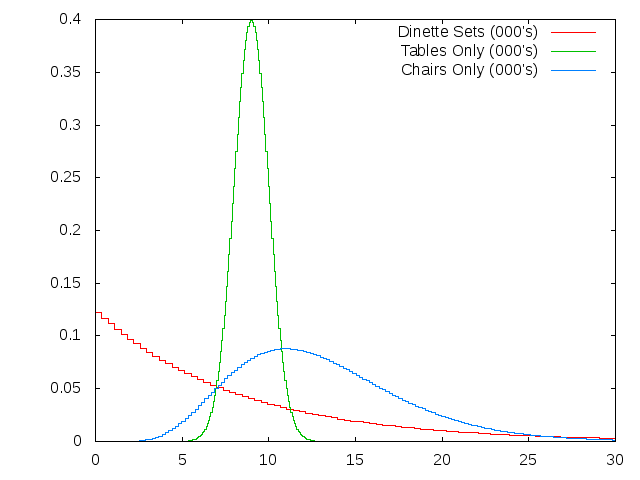
\includegraphics[width=120mm]{Images/TCD}
  \caption[Tables, Chairs and Dinette Sets Random Variables]
          {Tables, Chairs and Dinette Sets Random Variables}
  \label{fig:TCD}
\end{figure}

The manufacturer believes that market price and demand for tables are
related by the inverse function,

\begin{align*}
P_t = \frac{14*80}{D_t + D_d}
\end{align*}

where $D_t$ is the demand for tables alone and $D_d$ is the demand for
dinette sets. Thus $D_t + D_d$ is the total demand for tables. Similarly, the
price of chairs is related to the demand for chairs by the inverse
function,

\begin{align*}
P_c = \frac{24*45}{D_c + 2D_d}
\end{align*}

where $D_c$ is the demand for chairs alone and again $D_d$ is the
demand for dinette sets. The sale of one dinette set implies the sale
of two chairs. The actual functions are immaterial and have been
contrived so that the results of this version of the tables and chairs
example are comparable to previous versions. 

We recognize that $P_t$ and $P_c$ are correlated, but do not need to
materialize their joint probability distribution in order to compute
revenue results.

The example is data-intensive so we create some prototype software to
produce numerical results. Rather than presenting the prototype,
written in Python using the Numpy library, we describe the data
structures and sequence of operations.

Let our input random variables be,

\begin{align*}
Dt &= \{DXt, DPt\}\\
Dc &= \{DXc, DPc\}\\
Dd &= \{DXd, DPd\}
\end{align*}

where,

\begin{align*}
DXt &= (DXt_1, \dots, DXt_{Nt})\\
DPt &= (DPt_1, \dots, DPt_{Nt})\\
DXc &= (DXc_1, \dots, DXc_{Nc})\\
DPc &= (DPc_1, \dots, DPc_{Nc})\\
DXd &= (DXd_1, \dots, DXd_{Nd})\\
DPd &= (DPd_1, \dots, DPd_{Nd})
\end{align*}

and we assume that $DPt_{Nt} = DPc_{Nc} = DPd_{Nd} = 0$ as usual for
our numeric random variables since probability values are between
partition values. We have $Nt$, $Nc$ and $Nd$ as the number of
partition endpoints for each input random variable; tables, chairs and
dinette sets respectively.

We form the demand joint probability distribution $DP$ for the input random
variables by Cartesian product,

\begin{align*}
DP &= DPt \times DPc \times DPd
\end{align*}

We separately form parallel 3D arrays for each input demand,

\begin{align*}
DT &= DXt \times ones(Nc) \times ones(Nd)\\
DC &= ones(Nt) \times DXc \times ones(Nd)\\
DD &= ones(Nt) \times ones(Nc) \times DXd
\end{align*}

where, defining by example,

\begin{align*}
ones(5) = (1, 1, 1, 1, 1)
\end{align*}

Throughout this example presentation we will tend to use 2D diagrams
to represent 3D objects for clarity. In figure \ref{fig:tcd_rectangle} we
represent the demand joint probability $DP$ for a fixed value of $DXd$.

\begin{figure}
  \centering
  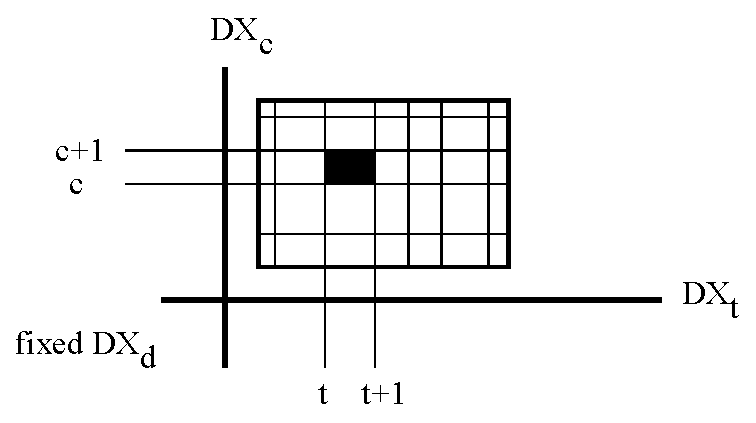
\includegraphics{Images/tcd_rectangle}
  \caption[One Layer of Demand Probability Array]
          {One Layer of Demand Probability Array}
  \label{fig:tcd_rectangle}
\end{figure}

In an abuse of notation, when no confusion arises, we use $t$, $c$ and
$d$ as both identifiers and indices. We then have the indices for
tables, chairs and dinette set random variables,

\begin{align*}
t &= 1 \dots Nt\\
c &= 1 \dots Nc\\
d &= 1 \dots Nd
\end{align*}

Now we can refer to a specific point within the demand joint
probability array as $DP_{t,c,d}$ or simply $DP_{tcd}$ where the commas are dropped for
clarity. The shaded rectangle in figure \ref{fig:tcd_rectangle} is
then the demand-space rectangular block of uniform probability
distribution with value $DP_{tcd}$.

The four 3D arrays $DT$, $DC$, $DD$ and $DP$ are all parallel. We will
now create other arrays parallel to these. The reason for this
parallelism is to ensure that the probability within each block is
correctly tracked through each step of the computation process.

The 3D arrays for the prices of tables and chairs are then written,

\begin{align*}
PT &= \frac{14*80}{DT + DD}\\
PC &= \frac{24*45}{DC + 2 DD}
\end{align*}

where the sums, $DT+DD$ and $DC + 2DD$, are computed element-wise as
well as the reciprocal functions. The result is that $PT$ and $PC$ are
3D arrays of size $Nt*Nc*Nd$ and are parallel to the demand and demand
probability arrays. Note in particular that the price arrays $PT$ and
$PC$ are not random variables. We will describe below how they may be
converted to random variable form. This is possible because we have
values of prices as vertices of a block of probability distribution
and we have the value of the probability uniformly distributed within
that block in the 3D array $DP$.

Now that we have our input prices the manufacturer may apply their
optimization and decide what combination of tables and chairs to
produce. In this example we have already computed the optimization
exhaustively and can therefore partition our demand space into the
three output cases $A$, $B$ and $C$. 

Consider that each point in the 3D demand array represents a
particular choice of input values that has associated with it two
particular prices, one for tables and the other for chairs. We have
already determined the rule for choosing each output case. We know,
for example, that if $\frac{2}{3}Pt < Pc$ then output $A$ will be
selected and similar rules apply for outputs $B$ and $C$. This means
for each point in our 3D demand we can assign a Boolean value $1$ or
$0$ where $1$ means that point has an associated price for chairs that
is larger then two-thirds that of tables. We can thus create a
parallel 3D array of Boolean values called a \emph{mask} based on the
optimized output selection rules. Let,

\begin{align*}
MA &= \frac{2}{3}PT < PC\\
MB &= \frac{1}{4}PT < PC < \frac{2}{3}PT\\
MC &= PC < \frac{1}{4}PT
\end{align*}

Each output is associated with some revenue. Using the price arrays
we can form parallel revenue arrays. Let,

\begin{align*}
RA &= 45PC\\
RB &= 24PC + 14PT\\
RC &= 20PT
\end{align*}

To convert  the revenue arrays, $RA$, $RB$ and $RC$ into random
variables we must first find a partition. We notice that while the
revenue arrays are parallel, using the masks we see that any given
point in the array space indexed by $(t,c,d)$ is intended to be
present in exactly one revenue array. This is because the output $A$,
$B$ and $C$ are mutually exclusive so, for example, the probability of
producing \$1000 and \$2000 of revenue using output $A$ can be added
to the probability of producing this same range of revenue for output
$B$ and for $C$ to arrive at a probability of producing that range of
revenue regardless of output choice. 

We would like the partition we use for the revenue random variable we
are about to produce to span the range of possible revenue values, be
fine where there is more revenue information and course where there is
less and be so fine overall that numerical artifacts overwhelm the
result. We chose for this example to use every $23^rd$ point from each
$175$-point input demand random variable and rerun the problem on the
partition values alone, not the probability values. In the Python code
this amounts to a single function call since all the code is in place
for the main computation. The result is are smaller versions over the
same revenue arrays representing collectively a sample of the possible
revenue values this example model produces using the given demand
inputs. The steps are as follows,

\begin{enumerate}
\item Form one dimensional arrays of valid revenue values for each
  output.
\item Run the same process as above to generate revenue arrays and
  output masks. Prepend an $s$ to the name indicating they are small
  versions due to the reduced partition size.
\item Concatenate the three 1D arrays into a single array called $temp$.
\item Sort the $temporary$ array and remove any duplicates.
\item append the value $-\infty$ to the start of the array and
  $\infty$ to the end. Call the result $Rx$.
\end{enumerate}

In this case the Python code from the prototype sums up the process concisely,

\begin{align*}
temp &= concatenate((sRA[sMA], sRB[sMB], sRC[sMC]))\\
Rx &= concatenate(([-\infty], unique(temp), [+\infty]))
\end{align*}

where $sRA[sMA]$ returns a one dimensional array from an arbitrary array
only for points where the corresponding point in the $sMA$ small
output mask array is a $1$ and $unique()$ sorts and removes duplicates
from an array. 

For each (big) output array $RA$, $RB$ and $RC$ with associated masks
$MA$, $MB$ and $MC$ we create a one dimensional array for the
probability distribution that is parallel to the one dimensional
partition array $Rx$. 

\begin{align*}
Rap &= zeros(Rx)\\
Rbp &= zeros(Rx)\\
Rcp &= zeros(Rx)
\end{align*}

where, defining by example,

\begin{align*}
zeros(5) = (0, 0, 0, 0, 0)
\end{align*}

The probability arrays, once filled in, will complete the formation of
the output revenue random variables,

\begin{align*}
Ra &= \{Rx, Rap\}\\
Rb &= \{Rx, Rbp\}\\
Rc &= \{Rx, Rcp\}
\end{align*}

The three output random variables $Ra$, $Rb$ and $Rc$ are mutually
exclusive and since they share a common partition we can add their
probability values to find the final output revenue random variable $R$,

\begin{align*}
R = \{Rx, Rap + Rbp + Rcp\}
\end{align*}

It remains to describe how to fill in the probability arrays $Rap$,
$Rbp$ and $Rcp$. We will describe the process for $Rap$ since it is
the same for the others.

Given the (big) output revenue 3D array $RA$, its associated mask
$MA$, the associated 3D probability array $DP$ and the 1D revenue
partition $Rx$ we proceed as follows to fill in the zero-valued 1D
probability array $Rap$. 

The output revenue 3D array $RA$ together with the associated
probability array $DP$ describes a partition of the joint demand
(input) space into blocks. Recall that we index the blocks with
indices $t$,$c$ and $d$ so that the $(t,c,d)$ block has uniform
probability $DP_{tcd}$ and eight vertices with the following revenues,

\begin{align*}
RA_{t,c,d} && RA_{t,c,d+1} && RA_{t,c+1,d} && RA_{t,c+1,d+1}\\
RA_{t+1,c,d} && RA_{t+1,c,d+1} && RA_{t+1,c+1,d} && RA_{t+1,c+1,d+1}
\end{align*}

for some block such that $1 \le t < Nt$, $1 \le c < Nc$ and $1 \le d <
Nd$. If all the vertices are \emph{valid}, that is, the associated
mask value is $1$ for each vertex then figure
\ref{fig:block_projection} symbolically represents one possible scenario.

\begin{figure}
  \centering
  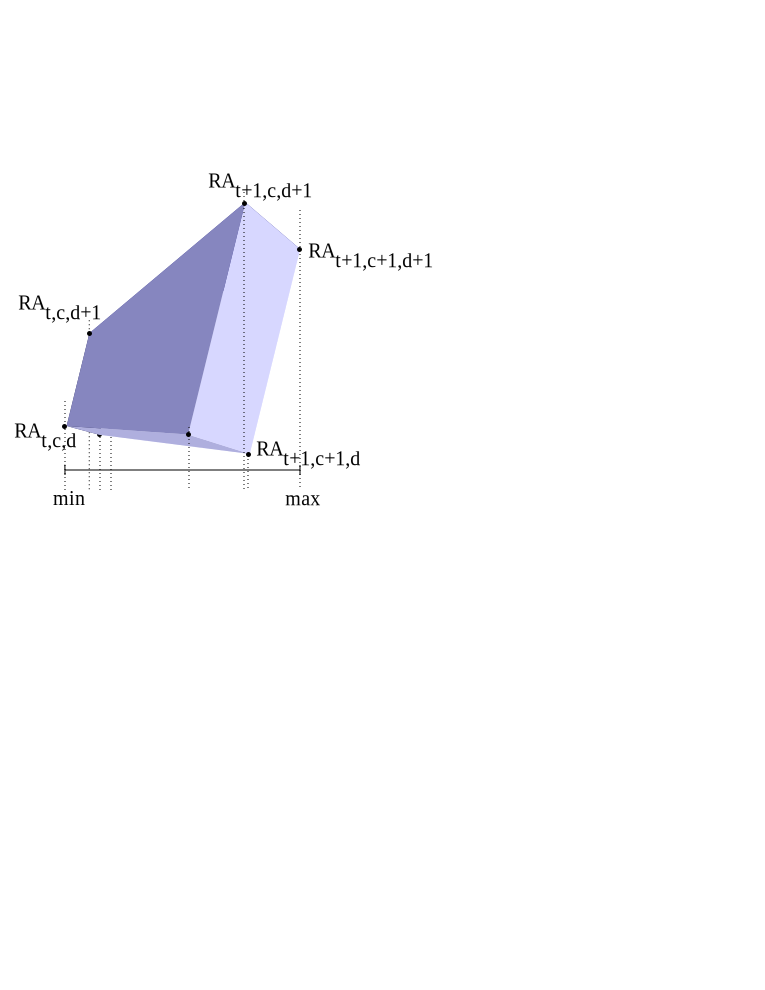
\includegraphics[width=3in]{Images/block_projection}
  \caption[Line Projection of 3D Probability Block]
          {Line Projection of 3D Probability Block}
  \label{fig:block_projection}
\end{figure}

The limits of the 3D block projection are the minimum and maximum
revenue vertex values. That is,

\begin{align*}
min_{tcd} &= Min(RA_{t,c,d}, \dots, RA_{t+1,c+1,d+1})\\
max_{tcd} &= Max(RA_{t,c,d}, \dots, RA_{t+1,c+1,d+1})
\end{align*}

For the software prototype version of this example we make the
assumption that the 3D block probability $DP_{t,c,d}$ is distributed
uniformly over the revenue line segment $(min, max)$ so that the
density is $h_{tcd}$,

\begin{align*}
h_{tcd} = \frac{DP_{tcd}}{max_{tcd} - max_{tcd}}
\end{align*}

where we have assumed that $min_{tcd} < max_{tcd}$. We will address
special cases such as when $min_{tcd}$ and $max_{tcd}$ are equal
below. Continuing with the general case we now allocate the
uniform probability density $h_{tcd}$ to the revenue probability array
$Rap$ recalling that $Rap$ is delimited by the partition array
$Rx$. Referring to figure \ref{fig:line_projection} we have,

\begin{figure}
  \centering
  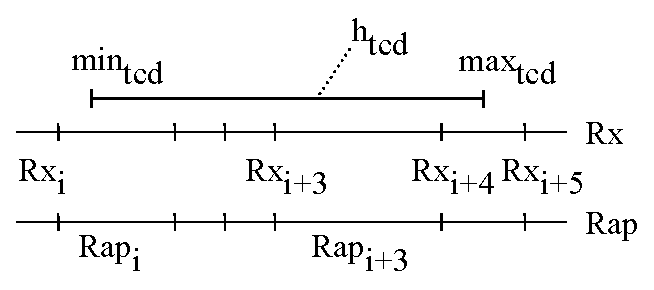
\includegraphics[width=3in]{Images/line_projection}
  \caption[Partition Allocation of Probability Line]
          {Partition Allocation of Probability Line}
  \label{fig:line_projection}
\end{figure}

\begin{align*}
Rap_i &= Rap_i + (Rx_{i+1} - min_{tcd}) h_{tcd}\\
\dots\\
Rap_{i+3} &= Rap_{i+3} + (Rx_{i+4} - Rx_{i+3}) h_{tcd}\\
Rap_{i+4} &= Rap_{i+4} + (max_{tcd} - Rx_{i+4}) h_{tcd} 
\end{align*}

where we have indicated how to compute end cases as well as cases
where $Rx$ partitions are spanned by the $(min_{tcd}, max_{tcd})$
interval. 

If the mask $MA$ indicates that some of the vertices of the $(t,c,d)$
block are not valid then we must reduce the amount of block
probability $DP_{tcd}$ available for allocation. For example, if $3$
of $8$ vertices are valid for the $(t,c,d)$ block then the block
probability is correspondingly reduced to $\frac{3}{8}DP_{tcd}$ so
that the $(min_{tcd}, max_{tcd})$ interval probability density is,

\begin{align*}
h_{tcd} = \frac{3}{8}\frac{DP_{tcd}}{max_{tcd} - max_{tcd}}
\end{align*}

If it happened that $min_{tcd} = max_{tcd}$ either because all the
valid vertices have the same revenue value or there is only one valid
vertex for the $(t,c,d)$ block then the corresponding partition
element is located for the $Rap$ array and its value is incremented
with the available probability for that block. If it happens that
$min_{tcd} = max_{tcd}$ equals an $Rx$ partition endpoint then the
available block probability is halved and allocated to the adjacent
partition intervals.

We perform the above operations for each output case and combine them
into the full revenue random variable and show the result in figure
\ref{fig:ABC_4}. The horizontal axis is dollars of revenue and vertical
axis is probability density as usual for random variable graphs. We
notice that the median value is roughly \$2200 because of careful
choice of demand inputs and the demand-to-price functional
relationship. 

%law of one price

\begin{figure}[ht]
\begin{minipage}[b]{0.5\linewidth}
\centering
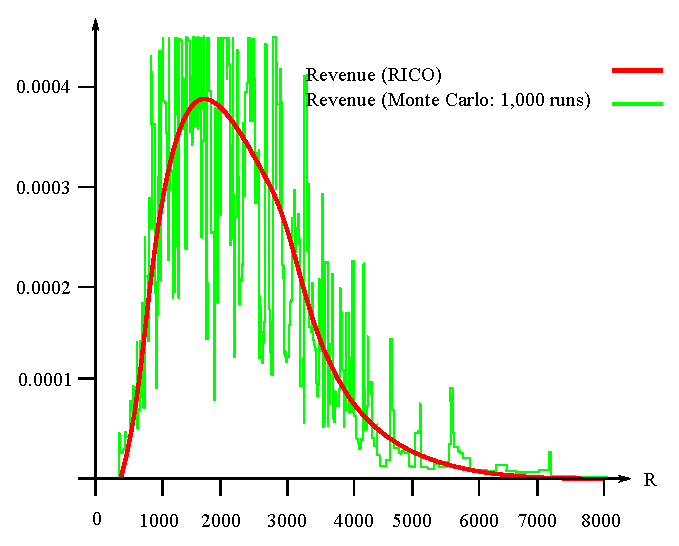
\includegraphics[width=2.33in, height=1.75in]{Images/ABC_1K}
\end{minipage}
\begin{minipage}[b]{0.5\linewidth}
\centering
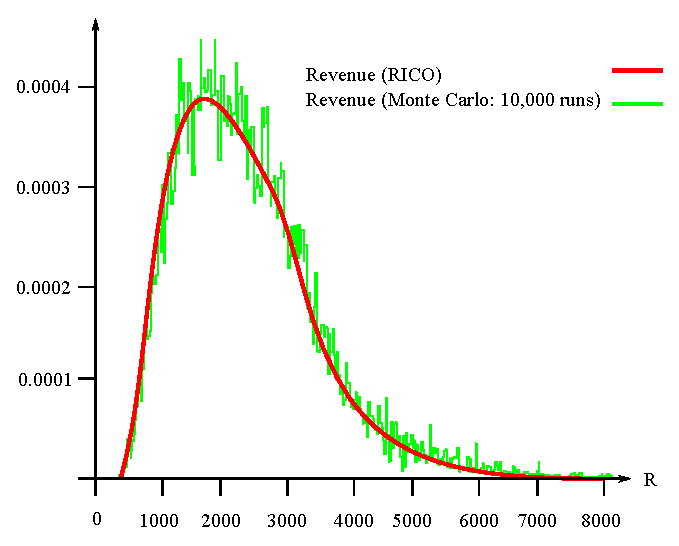
\includegraphics[width=2.33in, height=1.75in]{Images/ABC_10K}
\end{minipage}
\begin{minipage}[b]{0.5\linewidth}
\centering
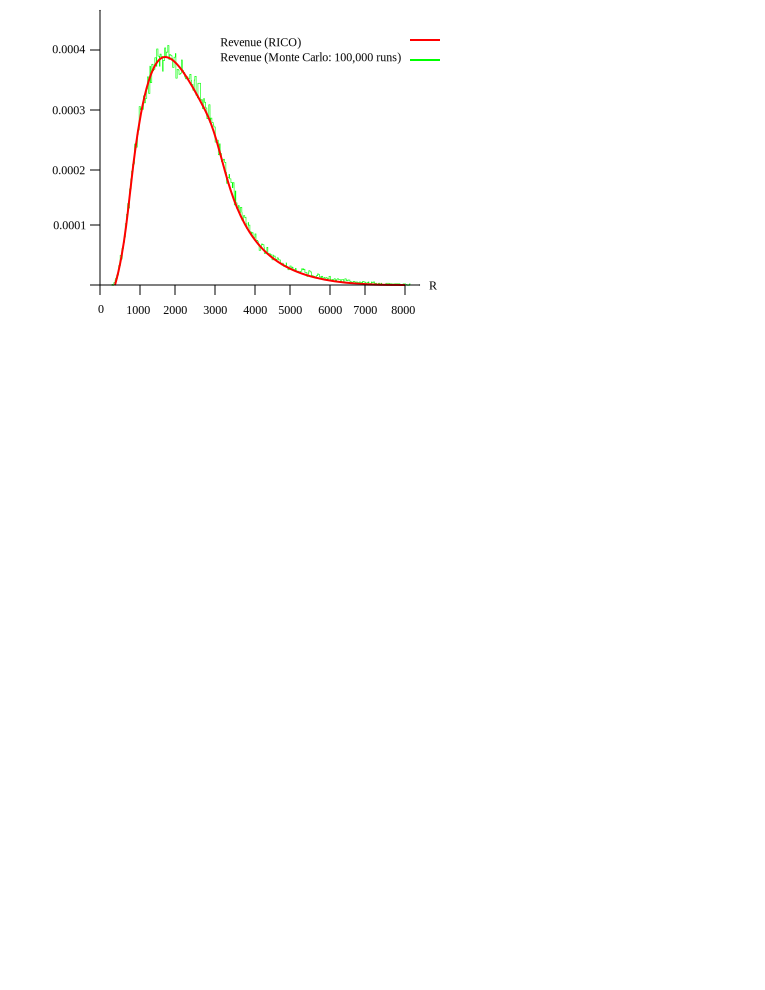
\includegraphics[width=2.33in, height=1.75in]{Images/ABC_100K}
\end{minipage}
\begin{minipage}[b]{0.5\linewidth}
\centering
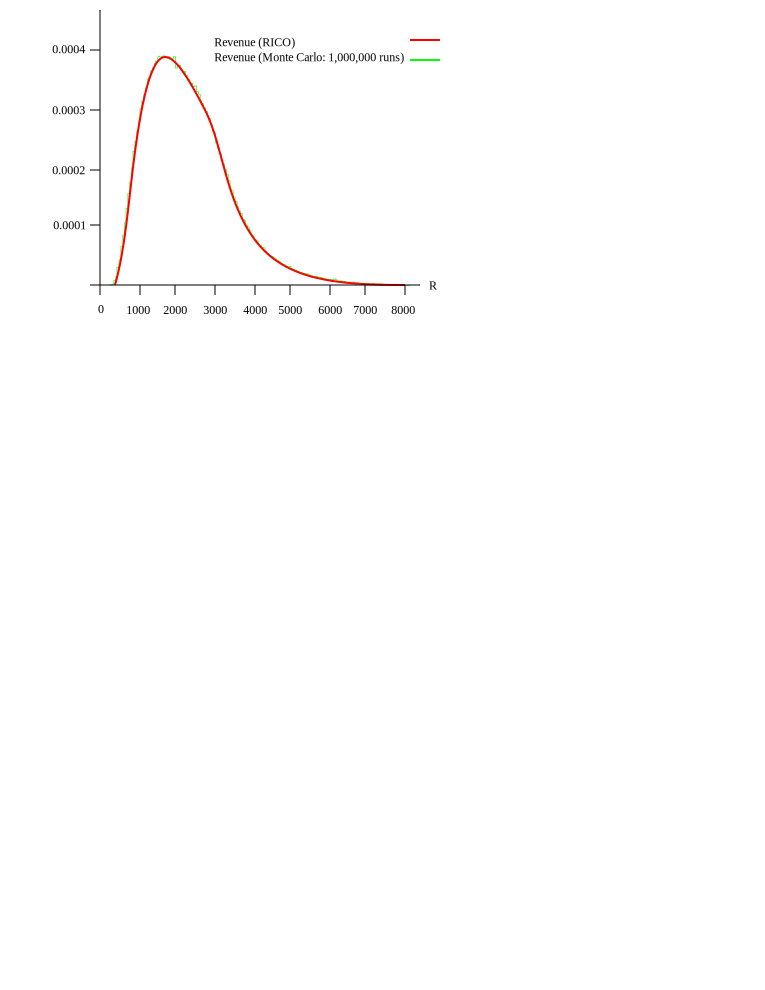
\includegraphics[width=2.33in, height=1.75in]{Images/ABC_1M}
\end{minipage}
  \caption[Random Revenue from Sales Combinations]
          {Random Revenue from Sales Combinations}
  \label{fig:ABC_4}
\end{figure}



Notable features of the optimized revenue in any panel of figure \ref{fig:ABC_4} is
that no matter what happens with the projected demand there is a
non-zero minimum revenue (about \$300), a strongly likelihood of
earning about \$2200 and significant possibility of earning
considerably more than the median \$2200.

We use the machinery developed above to convert the 3D price arrays to
random variables. Since there is no optimization involved in computing
prices there is no need to generate masks. Since we have some
information about the range of prices to expect we choose price
partitions directly. In this case each price is partitioned into
regularly spaced intervals from 0 to \$150. The
3D probability arrays are projected onto the price partitions and the
result for each price random variable is shown in figure
\ref{fig:tcd_prices}. Again we notice that, by design, the price of
chairs is has a median price of about \$45 and that of tables is about
\$80 which corresponds with the sharp version of the tables and chairs
example. 

\begin{figure}
  \centering
  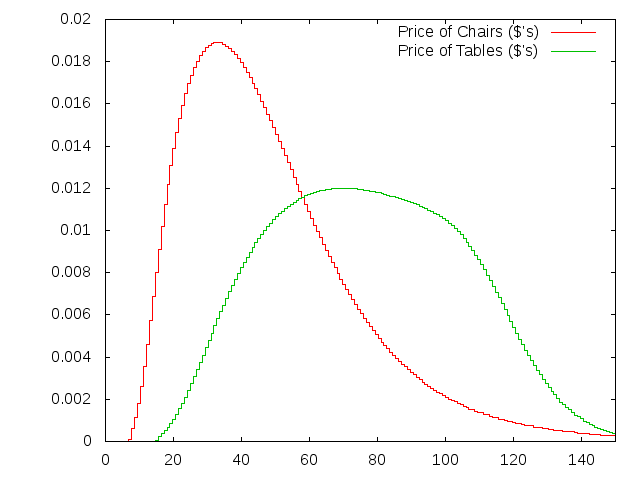
\includegraphics[width=120mm]{Images/tcd_prices}
  \caption[Random Variable Table and Chair Prices]
          {Random Variable Table and Chair Prices}
  \label{fig:tcd_prices}
\end{figure}

Notice that the price random variables are marginal probability
distributions for a joint probability distribution we have not
computed. Since the price for tables and chairs are non-trivially
correlated the joint distribution cannot be recovered from the
marginal distributions alone as described in a standard statistics
textbook such as \cite{bickel01}. 

\subsection{Finding the Joint Price Distribution from the Demand Inputs}

The reader will notice that we developed the tables and chairs example
with unknown prices in preparation for the introduction of random
inputs resulting in correlated prices we described how to proceed with
a joint distribution for the two prices, tables and chairs. Then we
solved the problem without using, or even finding, the joint price
distribution. Instead we used the 3D array created to represent the
three demand inputs. For this problem this technique provides directed
and satisfactory results.

In this section we revisit the tables and chairs example with the same
three demand input, but this time produce the joint price probability
distribution. Since so much of this work is devoted to the study of
correlated random variables we would be remiss not to include at least
one example of same.

We restart the problem with our three 3D demand arrays, $DT$, $DC$ and
$DD$. We also have the associated 3D probability array $DP$. Using the
same formulas as before for finding the (correlated) prices of tables
and chairs we produce the two 3D price arrays $PT$ and $PC$
respectively. 

This brings us to the point where we projected each 3D price array
onto a price partition and produced random variable representations of
the two prices in figure \ref{fig:tcd_prices}. We choose the same
price partitions as before, evenly space intervals from \$0 to
\$150. This choice allows us to compare the results we are about to
obtain with those obtained previously.

Our two price partitions, for $PT$ and $PC$, describe a 2D partition
of the $(Pc,Pt)$-space. If the number of points in each price
partition is $Np$ then we create a 2D array of size $Np^2$ and
initialize it with zero values.

We then realize that our two 3D price arrays $PT$ and $PC$ together
describe a 3D lattice of pairs of prices at each vertex surrounding a
uniform distribution of probability described by the 3D probability
array $DP$. The 8 vertices of each probability block, each containing the
two price values, are projected onto the two dimensional $(Pc,
Pt)$-space. This the 2D analog of our 1D procedure for finding each marginal
price random variable by projecting each price block for $PT$ or $PC$
onto the corresponding one dimensional price line. Figure
\ref{fig:ptc_rectangle} shows an example of price block vertex
projection. 

\begin{figure}
  \centering
  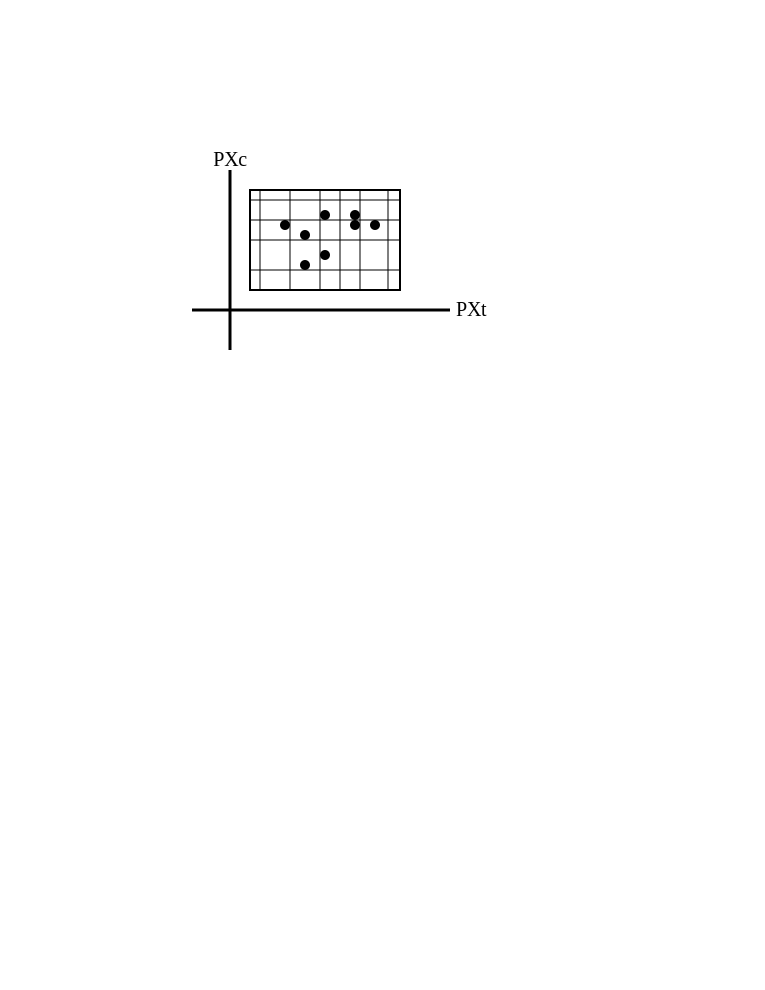
\includegraphics[width=3in]{Images/ptc_rectangle}
  \caption[Joint Price Partition with Block Vertex Projections]
          {Joint Price Partition with Block Vertex Projections}
  \label{fig:ptc_rectangle}
\end{figure}

Since the cluster of vertex projections in figure
\ref{fig:ptc_rectangle} indicate the projection of the 3D price
probability block onto the 2D joint price partition we must allocate
the block probability accordingly. 

Assuming that the cluster of vertex projections represent the limits
of the block projection we can find the convex hull of these points
using an algorithm such as the Graham 
Scan as described in a textbook of computer algorithms such as Corman
\cite{corman09}. We then assume the block probability is distributed
uniformly over the interior region of the convex hull and apportion it
accordingly to the partition rectangles of the 2D price
distribution, called $JP$. Figure \ref{fig:ptc_rectangle_convex} shows the convex
hull of the projected vertices. The heavy outline of joint price
rectangles shows the limits of affected rectangles. Let $p$ be the
probability of the projected block and $a$ the area of the convex
region, then $h = p/a$ is the probability density. The portion of
probability allocated to any given rectangle in the outlined region is
$h$ times the area of the rectangle intersecting the convex region.

\begin{figure}
  \centering
  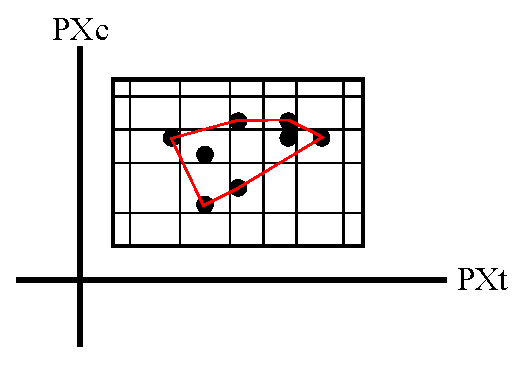
\includegraphics[width=3in]{Images/ptc_rectangle_convex}
  \caption[Joint Price Partition with Convex Block Projection]
          {Joint Price Partition with Convex Block Projection}
  \label{fig:ptc_rectangle_convex}
\end{figure}

In our running tables and chairs example we have over 5 million blocks
to project so we opt not to engage in a complex computation of
multiple rectangle intersections with convex regions associated with
each block, at least not for our prototype code. Instead we take a
simpler approach as shown in figure
\ref{fig:ptc_rectange_rectangle}. The heavy outline bounding box
represents the $Pt$ and $Pc$ partition limits bounding the block
vertex cluster. The shaded inner rectangle represents the rectangular
limits of the cluster points. We calculate the probability density of
the block probability if distributed uniformly over the inner shaded
rectangle and distribute this by area over each intersecting price
rectangle. 

\begin{figure}
  \centering
  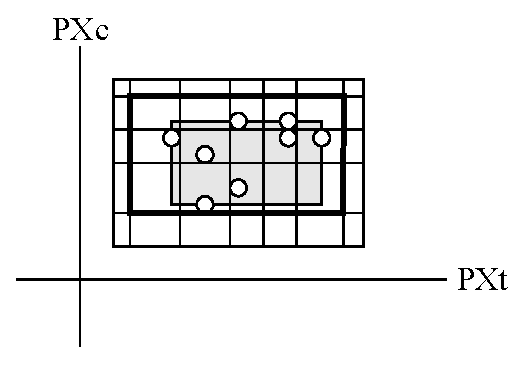
\includegraphics[width=3in]{Images/ptc_rectangle_rectangle}
  \caption[Joint Price Partition with Rectangular Block Projection]
          {Joint Price Partition with Rectangular Block Projection}
  \label{fig:ptc_rectange_rectangle}
\end{figure}

The results of the calculations of our prototype code for the joint
probability distribution of the two correlated prices is shown in
figure \ref{fig:Ptc}. Be aware that the origin is located in the
upper-left corner of the graph. The $x$ and $y$ axis are prices of
tables and chairs respectively and the vertical axis is probability density.

\begin{figure}
  \centering
  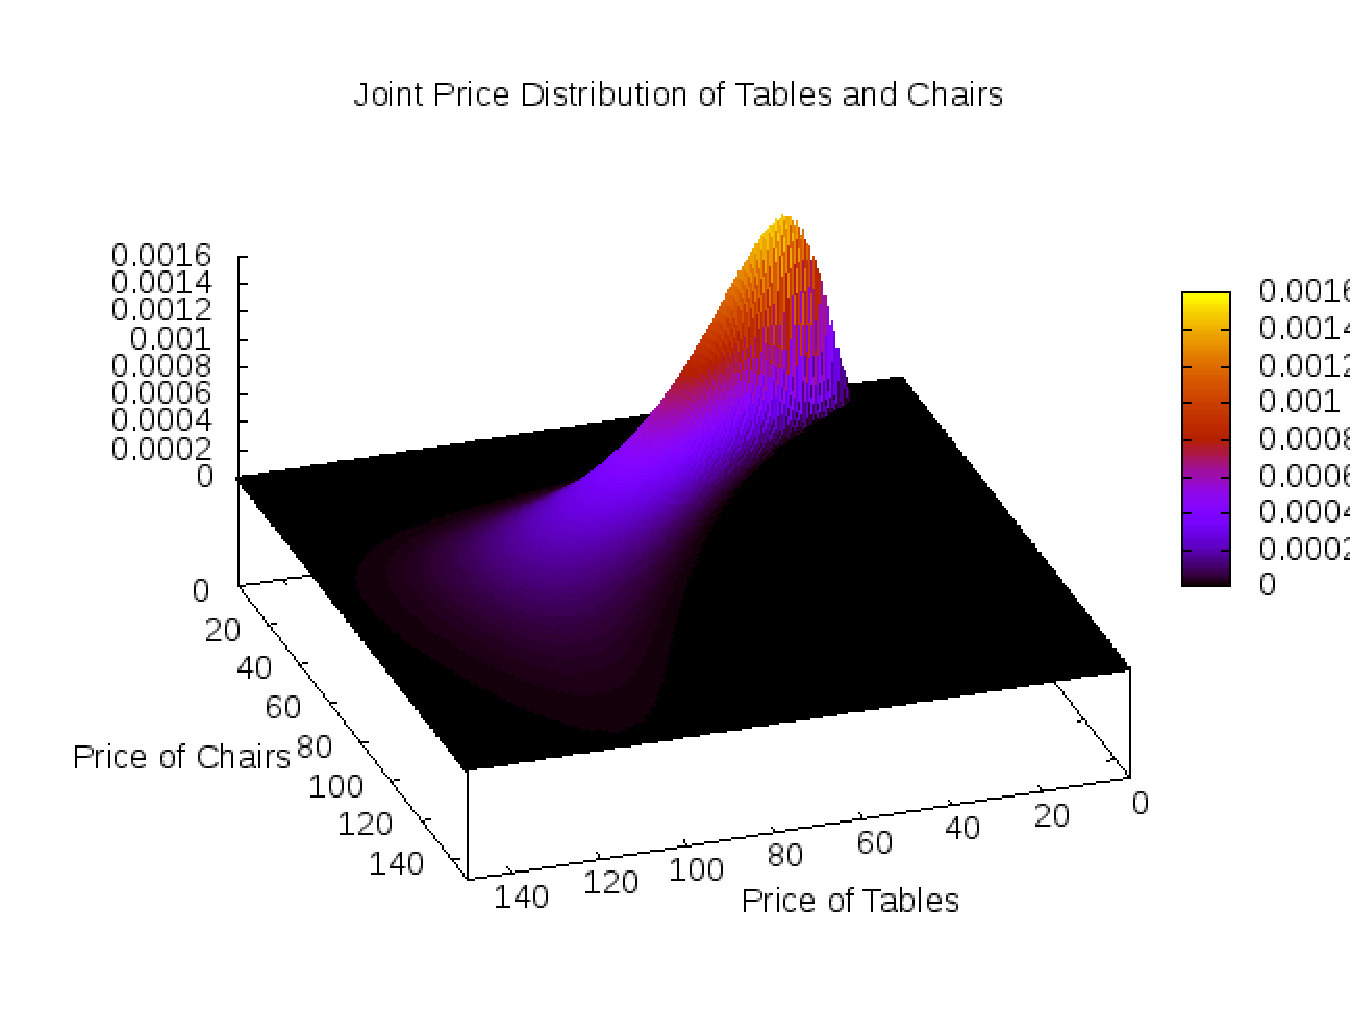
\includegraphics[width=120mm]{Images/Ptc.eps}
  \caption[Joint Probability Distribution of Table and Chair Prices]
          {Joint Probability Distribution of Table and Chair Prices}
  \label{fig:Ptc}
\end{figure}

An top view of the joint probability price distribution is
shown figure \ref{fig:Ptc_flat}. We compare this figure to our
original suggestion of the joint probability distribution of prices in
figure \ref{fig:tc_joint_prices}. 

\begin{figure}
  \centering
  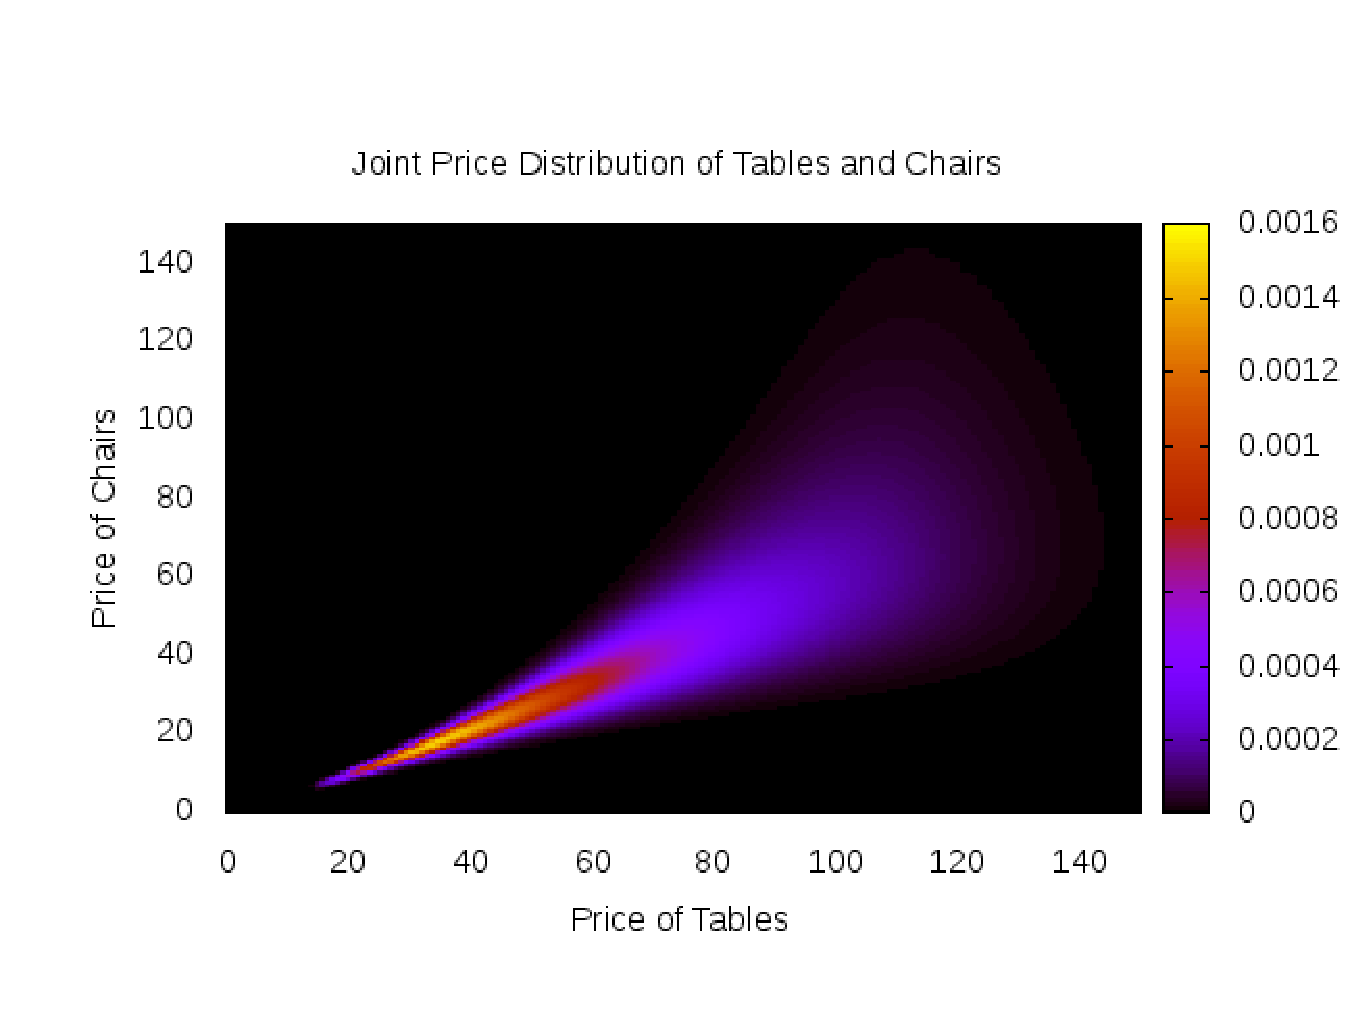
\includegraphics[width=120mm]{Images/Ptc_flat.eps}
  \caption[Joint Probability Distribution of Table and Chair Prices (Top View)]
          {Joint Probability Distribution of Table and Chair Prices (Top View)}
  \label{fig:Ptc_flat}
\end{figure}

It is interesting to note that the marginal random variable prices we
compute with the prototype code are identical to the random variable
price we computed previously and show in figure \ref{fig:tcd_prices}.

With the joint distribution of prices in hand we are able to address
the question of how to compute the probability of each branch in the
simplex graph (see figure \ref{fig:tc_directed_graph}). In particular
we are interested in the probabilities of the branch conditional
expressions,

\begin{align*}
p_t &< p_c\\
\frac{2}{3}p_t &< p_c\\
\frac{2}{3}p_t &< p_c < p_t\\
\frac{1}{4}p_t &< p_c\\
\frac{1}{4}p_t &< p_c < \frac{2}{3}p_t
\end{align*}

Proceeding as we did from the beginning, but starting with the jointly
distributed prices and their partitions $P_t$ and $P_c$ we create 2D
arrays $PT_2$ and $PT_2$ that are parallel to the 2D joint probability
distribution array $JP$. Taking the last inequality above as an
example we divide each expression by $p_t$ to find,

\begin{align*}
\frac{1}{4} < \frac{p_c}{p_t} < \frac{2}{3}
\end{align*}

In the prototype we form the 2D array expression $Qtc$ as,

\begin{align*}
Qtc = \frac{PC_2}{PT_2}
\end{align*}

as the element-wise quotient of the two 2D price arrays. We notice
that $Qtc$ together with the $JP$ form an improper form
two-dimensional random variable, a non-standard usage of the
expression. If we choose a 1D partition for $Qtc$ we can project our
$\{Qtc, JP\}$ pair onto this partition and find a proper-form random
variable, called $qtc$. As we have mentioned earlier, we address this case by
choosing the special partition,

\begin{align*}
Xqtc = (-\infty, 0, \frac{1}{4}, \frac{2}{3}, 1, \infty)
\end{align*}

The result is,

\begin{align*}
Pqtc = (0, 0.0001012, 0.7206, 0.2388, 0.03024, 0)
\end{align*}

Combining these into the random variable $Q$ for convenience as,

\begin{align*}
Q = \{Xqtc, Pqtc\}
\end{align*}

These probability values tell us probability of each simplex directed
graph branch and therefore the probability of each result. For
example, referring to figure \ref{fig:tc_directed_graph}, the
probability of taking the first left directed edge under the condition
that $p_t < p_c$ is  $\mathbb{P}(1 < Q) = 0.03024$. Similarly the
probability of reaching result $B$ is $\mathbb{P}(\frac{1}{4} < Q <
\frac{2}{3}) = 0.7206$.

\subsection{Tables and Chairs with Unknowns Prices and Resources}

If we allow prices and resources to be described by correlated random
variables the impact on the example is to increase the number of
branches from each simplex algorithm states and an increase in the
number of states. The simplex tableau for unknown prices and resources
is shown in table \ref{tab:pr0011}. 

\begin{table}
\centering
\begin{tabular}{| l | c c c c | c |}
\hline
0011    & $x_c$ & $x_t$ & $s_W$ & $s_L$ & $b$\\
\hline
$s_W$   & 5     & 20    & 1     & 0     & $b_W$\\
$s_L$   & 10    & 15    & 0     & 1     & $b_L$\\
\hline
Revenue & $p_c$    & $p_t$    & 0     & 0     &\\
\hline
\end{tabular}
  \caption[Tables and Chairs Simplex Tableau for Unknown Prices and Resources]
          {Tables and Chairs Simplex Tableau for Unknown Prices and Resources}
  \label{tab:pr0011}
\end{table}

The directed graph for the tables and chairs example
with unknown prices and resources is shown in figure
\ref{fig:tcpr_directed_graph}. Notice that there are only
$\mathbb{C}(4,2) = 6$ possible node states in this example. Notice
also that there are $5$ possible terminal states; manufacture of only
tables or only chair limited by either wood resource or labor resource
and also the mixed case.  

\begin{figure}
  \centering
  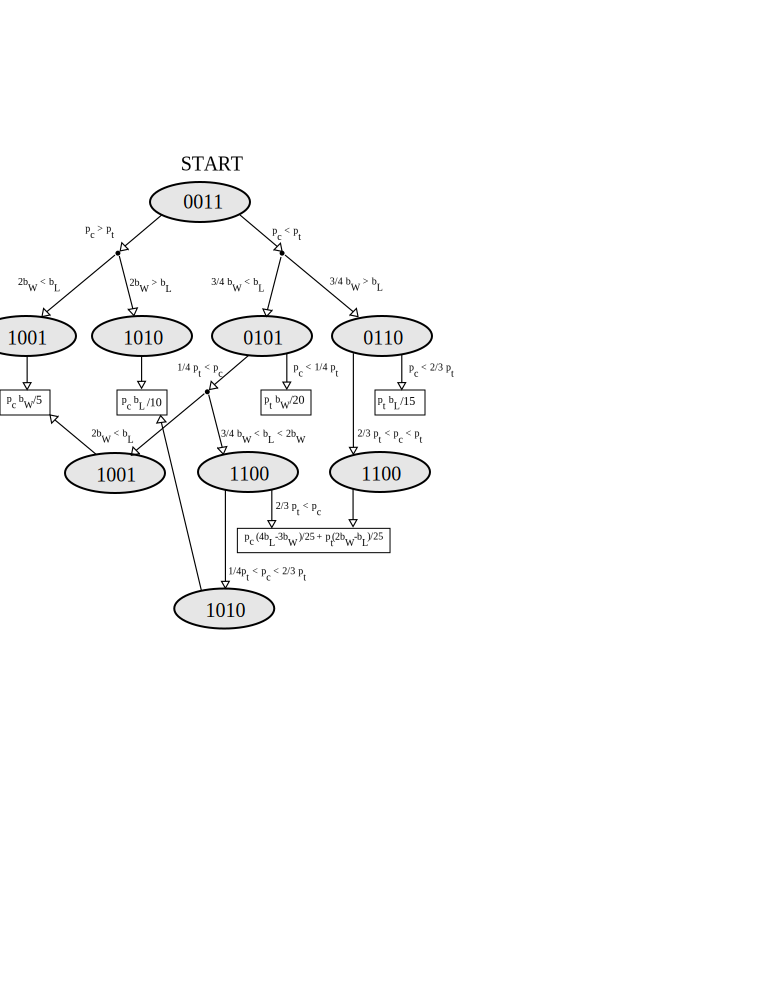
\includegraphics{Images/tcpr_directed_graph}
  \caption[Directed Graph for Tables and Chairs with Unknown Prices and Resources]
          {Directed Graph for Tables and Chairs with Unknown Prices and Resources}
  \label{fig:tcpr_directed_graph}
\end{figure}

While the conditions present when entering a state are significant,
the tableau in each state is denumerable as. We refer to tables
\ref{tab:pr1001}, \ref{tab:pr1010}, \ref{tab:pr0101}, \ref{tab:pr0110}
and \ref{tab:pr1100}. 

\begin{table}
\centering
\begin{tabular}{| l | c c c c | c |}
\hline
1001    & $x_c$ & $x_t$ & $s_W$ & $s_L$ & $b$\\
\hline
$s_W$   & 1     & 4      & $\frac{1}{5}$   & 0     & $\frac{b_W}{5}$\\
$s_L$   & 0     & -25    & -2              & 1     & $b_L - 2b_W$\\
\hline
Revenue & $p_c$    & $p_t$    & 0     & 0     &\\
\hline
\end{tabular}
  \caption[Tableau for Unknown Prices and Resources, State 1001]
          {Tableau for Unknown Prices and Resources, State 1001}
  \label{tab:pr1001}
\end{table}

\begin{table}
\centering
\begin{tabular}{| l | c c c c | c |}
\hline
1010    & $x_c$ & $x_t$ & $s_W$ & $s_L$ & $b$\\
\hline
$s_W$   & 1     & $\frac{3}{2}$  & 0   & $\frac{1}{10}$  & $\frac{b_L}{10}$\\
$s_L$   & 0     & -25            & 1   & -$\frac{1}{2}$  & $b_W - \frac{b_L}{2}$\\
\hline
Revenue & $p_c$    & $p_t$    & 0     & 0     &\\
\hline
\end{tabular}
  \caption[Tableau for Unknown Prices and Resources, State 1010]
          {Tableau for Unknown Prices and Resources, State 1010}
  \label{tab:pr1010}
\end{table}

\begin{table}
\centering
\begin{tabular}{| l | c c c c | c |}
\hline
0101    & $x_c$ & $x_t$ & $s_W$ & $s_L$ & $b$\\
\hline
$s_W$   & $\frac{1}{4}$   & 1  & $\frac{1}{20}$   & 0  & $\frac{b_W}{20}$\\
$s_L$   & $\frac{25}{4}$  & 0  & -$\frac{3}{4}$   & 1  & $b_L - \frac{3}{4}b_W$\\
\hline
Revenue & $p_c$    & $p_t$    & 0     & 0     &\\
\hline
\end{tabular}
  \caption[Tableau for Unknown Prices and Resources, State 0101]
          {Tableau for Unknown Prices and Resources, State 0101}
  \label{tab:pr0101}
\end{table}

\begin{table}
\centering
\begin{tabular}{| l | c c c c | c |}
\hline
0110    & $x_c$ & $x_t$ & $s_W$ & $s_L$ & $b$\\
\hline
$s_W$   & $\frac{2}{3}$    & 1  & 0  & $\frac{2}{30}$  & $\frac{b_L}{15}$\\
$s_L$   & -$\frac{25}{3}$  & 0  & 1  & -$\frac{4}{3}$  & $b_W - \frac{4}{3}b_L$\\
\hline
Revenue & $p_c$    & $p_t$    & 0     & 0     &\\
\hline
\end{tabular}
  \caption[Tableau for Unknown Prices and Resources, State 0110]
          {Tableau for Unknown Prices and Resources, State 0110}
  \label{tab:pr0110}
\end{table}

\begin{table}
\centering
\begin{tabular}{| l | c c c c | c |}
\hline
1100    & $x_c$ & $x_t$ & $s_W$ & $s_L$ & $b$\\
\hline
$s_W$   & 1  & 0  & -$\frac{3}{25}$  & $\frac{4}{25}$  & $\frac{4b_L-3b_W}{25}$\\
$s_L$   & 0  & 1  & $\frac{2}{25}$  & -$\frac{1}{25}$  & $\frac{2b_W-b_L}{25}$\\
\hline
Revenue & $p_c$    & $p_t$    & 0     & 0     &\\
\hline
\end{tabular}
  \caption[Tableau for Unknown Prices and Resources, State 1100]
          {Tableau for Unknown Prices and Resources, State 1100}
  \label{tab:pr1100}
\end{table}

Starting in state $0011$ we follow the simplex two-phase decision and
first compare the two prices $p_c$ and $p_t$. We are assuming for
clarity, as before, that since we intend to replace $p_c$ and $p_t$
with continuous random variables the probability of equality is
zero. In practice we need to check for the possibility of
equality. The initial comparisons are,

\begin{align*}
argmax(p_c, p_t)\\
argmin(\frac{b_W}{5}, \frac{b_L}{10}  | > 0 \text{ and } p_c > p_t)\\
argmin(\frac{b_W}{20}, \frac{b_L}{15} | > 0 \text{ and } p_c < p_t)
\end{align*}

where the $> 0$ condition refers to the requirement that each operand
be positive else it is disqualified from the comparison.

%4/21/2011 p.2

In many cases the first or second phase of the simplex algorithm
decision is disqualified since it is either non-positive or contradicts
a previous assumption. 

Since simplex states may be re-entered a computer algorithm can take
advantage of this possibility and cache, rather than recompute, certain
elements such as the simplex tableau. At each decision point we see
again that we are comparing linear combinations of either price or
resource variables with zero in the sense that the expression $a < b$
can be rewritten as $0 < b - a$. We have seen in the previous version
of the tables and chairs example that each conditional statement
results in a filter on the input space so that the simplex algorithm
may be viewed as a filtration process. The task of the RICO modeling
environment is to determine what portion of the input space passes through
each facet of the simplex filtration process to a terminal node and
with what probability.

\section{Beyond the Tables and Chairs Example}

In the tables and chairs example we chose correlated random inputs for
prices and argued that we could have chosen correlated random inputs
for resources instead. We notice in the simplex algorithm the
transition decision from one state to the other involves computing the
maximum positive revenue impact in the case of prices and then the
minimum positive resource impact. These two choices correspond to the
two facets of a table pivot as explained above. 

It remains to be investigated what happens to this example when some
or all of the values of $A$ are unknown. In this example the
significance of unknown $A$ values is that the manufacturer is unsure
how many resources are consumed by each product.

As explained by Bellman \cite{bellman03}, the number of solution
states, not to mention the number of internal simplex algorithm
states, becomes computationally intractable even for modest
problems. We see this for ourselves if the problem has 100 variables
and 100 constraints then the number of simplex states is at least
$\mathbb{Ch}(200,100) = 9.05\times10^{58}$. The reference implementation
of the AB32 model has many hundreds of variables and several thousand
constraint equations. 

A way to proceed is for the RICO modeling environment to partially explore
the simplex directed graph. The transition from one state to the next
using the simplex algorithm involves finding the maximum of a set of
linear combinations of prices, in the context of the tables and chairs
example, followed by finding the minimum of a set of linear
combinations of resource limits assuming the $A$ values are fixed. As
we have seem each \emph{choice element} is a linear combination of random
variables which are themselves random variables. If we assume there
are three choice elements denoted $X$, $Y$ and $Z$ then the decision,

\begin{align*}
argmax\{X, Y, Z\}
\end{align*}

results in three probability values,

\begin{align*}
\mathbb{P}(X < \{Y, Z\})\\
\mathbb{P}(Y < \{X,Z\})\\
\mathbb{P}(Z < \{X,Y\})
\end{align*}

In this case the simplex algorithm state has three initial branches
corresponding to the first decision of the pivot element. These
probabilities may be computed explicitly and rather than create a
directed graph with all choices listed as we did above with the tables
and chairs directed graph, we choose only the most highest probability
transition. In this manner we reach a terminal node as in the sharp
version of the simplex algorithm. 

Since we are able to assign probability values to each transition edge
in the directed graph we may apply a choice algorithm to explore other
paths based on their likelihood of occurrence. As long as the directed
graph remains at least partly unexplored, we suspect this is the case
in general, then the random variable results will not have \emph{full
  probability}, that is, their probability values will sum to less
than one. The proximity of the probability sum of a random variable
result to unity can be used as a criterion for algorithm
termination. That is, if the random variable result is deemed near
enough to completion the algorithm can terminate its exploration
of the simplex directed graph.
 
